\documentclass[conference]{IEEEtran}

\usepackage[T1]{fontenc}
\usepackage[utf8]{inputenc}
\usepackage[brazil]{babel}
\usepackage{cite}
\usepackage{amsmath, amssymb, mathtools}
\usepackage{graphicx}
\usepackage{booktabs}
\usepackage{url}

\graphicspath{{imagens/}}   % figuras ficam na pasta imagens/ (as mesmas da apresentação)
\renewcommand{\IEEEkeywordsname}{Palavras-chave}
\addto\captionsbrazil{\renewcommand{\figurename}{Fig.}}   % legenda no padrão IEEE (Fig.)

\begin{document}

\title{Aprendizado por Reforço Aplicado a \textit{Trading} de Bitcoin: \textit{Value Iteration}, Monte Carlo e Q-learning}

\author{\IEEEauthorblockN{Tiago Macedo, Viktor Mayer e Enzo Guedes}
\IEEEauthorblockA{IBMEC\\
Professor: Rodrigo Luna}}

\maketitle

% =============================================================
\begin{abstract}
Este trabalho modela a decisão diária de \textit{trading} em Bitcoin (BTC-USD) como um Processo de Decisão de Markov finito de 27 estados. O estado combina o desvio do preço em relação à média móvel de 50 dias, hoje e ontem, e a posição mantida. A recompensa é o log-retorno da carteira, já descontada a corretagem, de modo que a soma das recompensas é o log do patrimônio final. O problema é resolvido por três métodos: \textit{Value Iteration} sobre um modelo estimado empiricamente e, sem modelo, Monte Carlo e Q-learning. Tudo é aprendido com dados de 2014 a 2021, e as políticas são avaliadas fora da amostra, de 2022 a 2026, no simulador \texttt{gym-trading-env}. Com corretagem de 0,1\%, o \textit{Value Iteration} obteve índice de Sharpe de 0,46 e \textit{drawdown} máximo de $-29{,}35\%$, contra 0,04 e $-66{,}93\%$ do \textit{Buy \& Hold}. O Monte Carlo chegou a 0,44 sem conhecer o modelo, e o Q-learning a 0,26. As três políticas superaram seis modelos econométricos de previsão de retornos em Sharpe e Calmar. Uma validação \textit{walk-forward} mostrou que retreinar periodicamente com todo o histórico não melhorou nenhum modelo, e uma bateria de fatores de desconto, avaliada sem usar o teste, sustentou a escolha $\gamma = 0{,}8$.
\end{abstract}

\begin{IEEEkeywords}
Aprendizado por reforço, processo de decisão de Markov, \textit{Value Iteration}, Monte Carlo, Q-learning, \textit{trading} algorítmico, Bitcoin.
\end{IEEEkeywords}

% =============================================================
\section{Introdução}

O aprendizado por reforço (\textit{reinforcement learning}, RL) estuda agentes que aprendem a agir por tentativa e erro, maximizando uma recompensa acumulada ao longo do tempo~\cite{sutton2018}. Em finanças, a formulação é natural: a cada dia o agente escolhe uma posição, o mercado responde com um retorno e a carteira acumula o resultado, descontados os custos de transação~\cite{moody1998,moody2001}.

Este trabalho aplica três métodos clássicos de RL tabular a um problema deliberadamente simples, a negociação diária de Bitcoin com posições vendida, neutra e comprada. O objetivo é comparar, nas mesmas condições, a solução com modelo (\textit{model-based}) e as soluções sem modelo (\textit{model-free}). As contribuições são:
\begin{itemize}
  \item um MDP de 27 estados cuja recompensa é o log-retorno da carteira, de forma que maximizar o retorno acumulado equivale a maximizar o crescimento do patrimônio;
  \item a solução desse MDP por \textit{Value Iteration} sobre um modelo estimado e por Monte Carlo e Q-learning sem modelo, com análise de convergência e de variabilidade entre sementes;
  \item a avaliação fora da amostra no simulador \texttt{gym-trading-env}~\cite{gymtrading}, com referências simples, modelos econométricos, validação \textit{walk-forward} e escolha do fator de desconto sem usar o período de teste.
\end{itemize}

A Seção~\ref{sec:formulacao} formula o problema e a Seção~\ref{sec:mdp} define estado, ação e recompensa. A Seção~\ref{sec:modelo} descreve a estimação do modelo e o \textit{Value Iteration}, e a Seção~\ref{sec:modelfree} apresenta Monte Carlo e Q-learning. A Seção~\ref{sec:metodologia} detalha o protocolo experimental, a Seção~\ref{sec:resultados} reporta os resultados, a Seção~\ref{sec:discussao} os discute e a Seção~\ref{sec:conclusao} conclui.

% =============================================================
\section{Formulação do Problema}
\label{sec:formulacao}

O problema de negociação é modelado como um Processo de Decisão de Markov (MDP)~\cite{puterman1994,sutton2018}
\begin{equation}
  \mathcal{M} = (\mathcal{S}, \mathcal{A}, P, R, \gamma),
\end{equation}
em que $\mathcal{S}$ é o espaço de estados, $\mathcal{A}$ o espaço de ações, $P$ a dinâmica de transição, $R$ a recompensa e $\gamma$ o fator de desconto. O objetivo do agente é encontrar uma política ótima $\pi^*$ que maximize o retorno esperado acumulado:
\begin{equation}
  \pi^* = \arg\max_{\pi} \mathbb{E}_{\pi}[G_0].
\end{equation}

Como a recompensa é a variação logarítmica do patrimônio $W_t$ (Seção~\ref{sec:recompensa}), o retorno acumulado a partir do instante $t$ é
\begin{equation}
  G_t = \sum_{k=0}^{T-t-1} \gamma^k \ln\frac{W_{t+k+1}}{W_{t+k}},
  \label{eq:retorno}
\end{equation}
em que $T$ é o instante final do episódio. No caso não descontado ($\gamma = 1$), a soma é telescópica e $G_t = \ln(W_T / W_t)$ é exatamente o log-retorno total da carteira no período restante. Maximizar o valor esperado dessa quantidade equivale ao critério de Kelly~\cite{kelly1956}, isto é, à maximização da taxa de crescimento composto do capital.

Na solução por programação dinâmica (Seção~\ref{sec:vi}), o modelo estimado é tratado como estacionário e de horizonte infinito, o que exige $\gamma \in [0, 1)$ para garantir a convergência. Quanto mais próximo de $1$, mais $G_t$ se aproxima do log-retorno total da carteira. A escolha $\gamma = 0{,}8$ é discutida na Seção~\ref{sec:gamma}.

% =============================================================
\section{Estado, Ação e Recompensa}
\label{sec:mdp}

\subsection{Dados}

Os preços diários de fechamento do BTC-USD foram obtidos do Yahoo Finance com a biblioteca \texttt{yfinance}~\cite{yfinance}. O Bitcoin negocia 24 horas por dia, sete dias por semana. O fechamento diário corresponde a 0h UTC (21h de Brasília), e um ano tem 365 períodos nas métricas. O treino vai de 06/11/2014 a 31/12/2021, e o teste, de 01/01/2022 a 18/11/2026 (1.783 dias). A data final é fixa, de modo que todos os resultados são reproduzíveis. Toda estimação usa apenas o treino; o teste é usado uma única vez, ao final.

\subsection{Retornos e Sinal de Tendência}

Seja $c_t$ o preço de fechamento no dia $t$. Os retornos logarítmico e simples do ativo são~\cite{campbell1997,tsay2010}
\begin{equation}
  \rho_t = \ln\frac{c_t}{c_{t-1}}, \qquad r_t = \frac{c_t}{c_{t-1}} - 1.
\end{equation}
O estado não usa o retorno diário, mas um sinal de tendência: o desvio logarítmico do preço em relação à média móvel de 50 dias,
\begin{equation}
  x_t = \ln\frac{c_t}{\mathrm{MA}_{50}(c_t)},
\end{equation}
positivo quando o preço está acima da média e negativo quando está abaixo. O estado contínuo de observação é
\begin{equation}
  s_t = (x_t,\, x_{t-1},\, h_{t-1}),
\end{equation}
em que o par $(x_t, x_{t-1})$ captura o nível e a direção recente da tendência, e $h_{t-1}$ é a posição (do inglês \textit{holding}) mantida pelo agente no dia anterior. A inclusão de $h_{t-1}$ é necessária para que o custo de transação, que depende da mudança de posição, seja função do estado e da ação.

\subsection{Espaço de Ações}

O agente escolhe a posição a ser assumida no mercado:
\begin{equation}
  \mathcal{A} = \{-1, 0, +1\}, \qquad h_t = a_t, \qquad a_t \in \mathcal{A}.
\end{equation}
As ações correspondem, respectivamente, às posições vendida (\textit{short}), neutra (fora do mercado) e comprada (\textit{long}).

\subsection{Função de Recompensa}
\label{sec:recompensa}

Seja $\kappa \ge 0$ a corretagem proporcional, cobrada por unidade de posição negociada; neste trabalho, $\kappa = 0{,}1\%$. A ação $a_t$ é decidida no fechamento do dia $t$, e o patrimônio evolui segundo~\cite{moody1998,moody2001}
\begin{equation}
  \frac{W_{t+1}}{W_t} = 1 + a_t\, r_{t+1} - \kappa\, |a_t - h_{t-1}|.
\end{equation}
Como $|a_t - h_{t-1}| \in \{0, 1, 2\}$, entrar ou sair de uma posição custa $\kappa$, e inverter diretamente de comprado para vendido (ou o contrário) custa $2\kappa = 0{,}2\%$. A recompensa imediata é o log-retorno da carteira:
\begin{align}
  R_{t+1} &= \ln\frac{W_{t+1}}{W_t} \nonumber \\
          &= \ln\!\big(1 + a_t\, r_{t+1} - \kappa\, |a_t - h_{t-1}|\big).
  \label{eq:recompensa}
\end{align}
O uso do retorno simples $r_{t+1}$ dentro do logaritmo trata corretamente a posição vendida, pois $\ln(1 - r) \neq -\ln(1 + r)$. A recompensa é invariante à escala do capital: sua magnitude independe do volume financeiro acumulado.

\subsection{Discretização do Estado}

Para viabilizar a solução tabular, o sinal contínuo é mapeado em três faixas:
\begin{equation}
  \phi(x) =
  \begin{cases}
    0 \ (\text{baixa}),  & x \le \tau_1, \\
    1 \ (\text{neutro}), & \tau_1 < x \le \tau_2, \\
    2 \ (\text{alta}),   & x > \tau_2,
  \end{cases}
\end{equation}
em que os limiares são os tercis empíricos de $x_t$, calculados exclusivamente no treino:
\begin{equation}
  \tau_1 = Q_{1/3}(x_{\mathrm{treino}}), \qquad \tau_2 = Q_{2/3}(x_{\mathrm{treino}}).
\end{equation}
Com os 2.614 valores de $x_t$ do treino, obtém-se $\tau_1 = -0{,}0234$ (preço 2,3\% abaixo da média) e $\tau_2 = 0{,}0953$ (10\% acima). Os limiares não são simétricos porque, no treino, o BTC passou mais tempo acima da média (Fig.~\ref{fig:tercis}). O teste usa os mesmos limiares, sem recalculá-los. As faixas são equiprováveis apenas no treino; no teste, mudanças de regime podem alterar a frequência de cada uma.

\begin{figure}[!t]
  \centering
  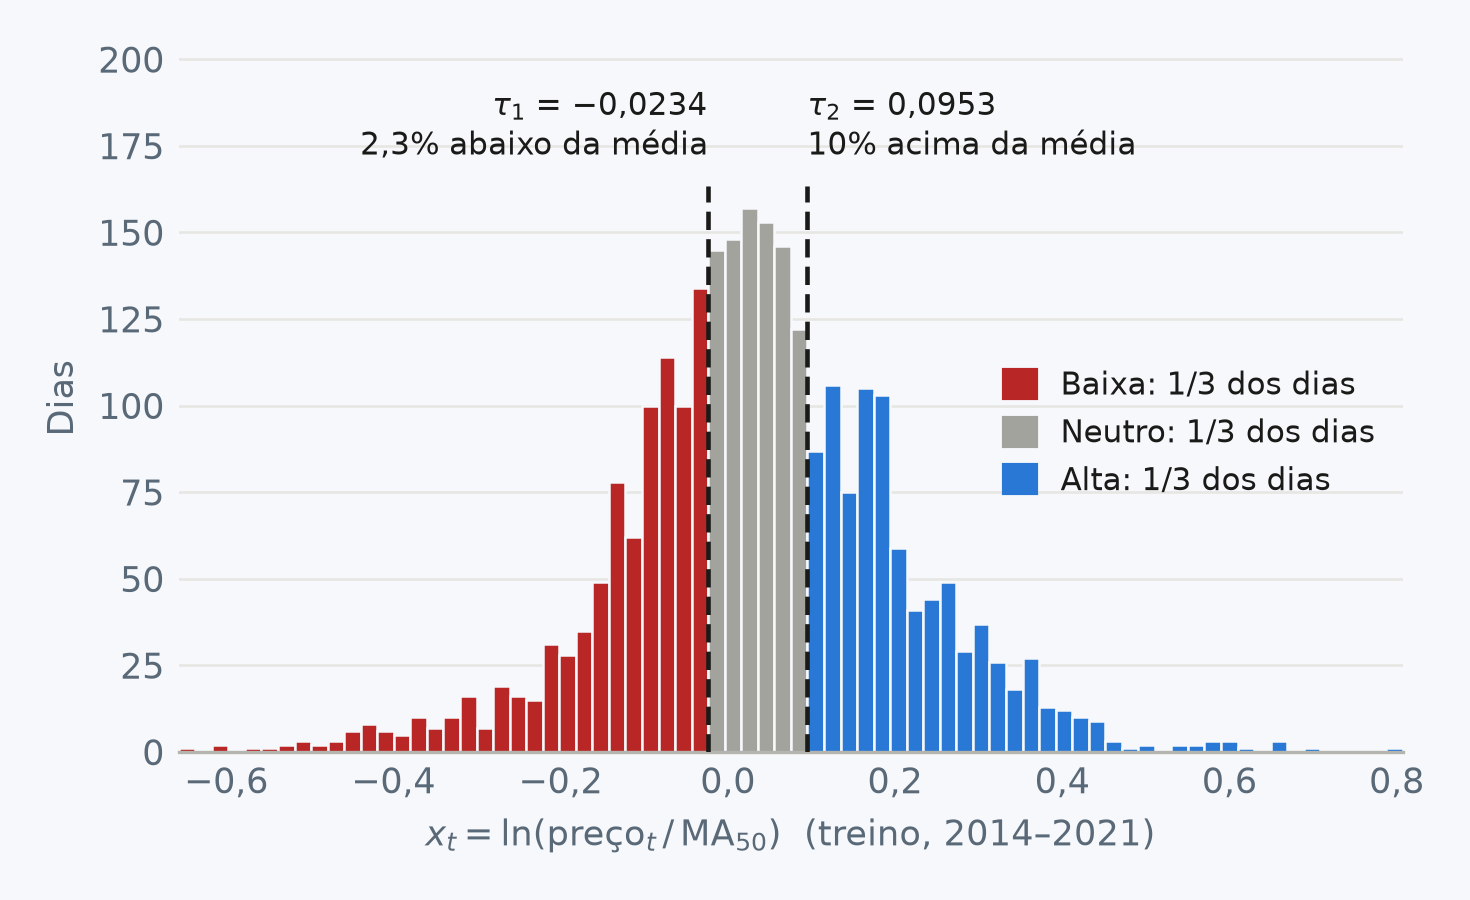
\includegraphics[width=\columnwidth]{limiares_tercis.png}
  \caption{Distribuição de $x_t$ no treino (2014--2021). Os limiares $\tau_1$ e $\tau_2$ dividem os dias em três faixas com 1/3 dos dias cada.}
  \label{fig:tercis}
\end{figure}

O estado discreto é
\begin{equation}
  \tilde{s}_t = \big(\phi(x_t),\, \phi(x_{t-1}),\, h_{t-1}\big),
\end{equation}
e os espaços de estados e ações ficam
\begin{equation}
  \mathcal{S} = \{0,1,2\}^2 \times \{-1, 0, +1\}, \quad |\mathcal{S}| = 27, \quad |\mathcal{A}| = 3.
\end{equation}
A mesma discretização é usada pelos três métodos. A propriedade de Markov é uma aproximação: nada garante que os 27 estados resumam toda a informação relevante do passado do mercado. Essa hipótese pesa de forma diferente sobre cada método (Seção~\ref{sec:modelfree}).

% =============================================================
\section{Modelo Estimado e \textit{Value Iteration}}
\label{sec:modelo}

\subsection{Funções de Valor}

Para uma política $\pi$, as funções valor de estado e de ação são
\begin{align}
  V^\pi(s)   &= \mathbb{E}_\pi\left[G_t \;\middle|\; S_t = s\right], \\
  Q^\pi(s,a) &= \mathbb{E}_\pi\left[G_t \;\middle|\; S_t = s,\, A_t = a\right].
\end{align}
$V^\pi(s)$ mede o log-crescimento esperado do patrimônio a partir do estado $s$, e $Q^\pi(s,a)$ indica se assumir posição comprada, vendida ou neutra produz o maior crescimento esperado. Uma política é uma distribuição $\pi(a \mid s)$ sobre as ações, e as duas funções se relacionam por $V^\pi(s) = \sum_{a} \pi(a \mid s)\, Q^\pi(s,a)$.

\subsection{Estimação das Probabilidades de Transição}

Como o agente não influencia o preço, a única parte aleatória da transição é a próxima faixa $j = \phi(x_{t+1})$, que depende das faixas de hoje, $i = \phi(x_t)$, e de ontem, $k = \phi(x_{t-1})$. A parte da posição é determinística: a próxima posição é a própria ação. A probabilidade é estimada por frequência relativa no treino, que é o estimador de máxima verossimilhança das probabilidades de transição de uma cadeia de Markov~\cite{anderson1957}. Seja $N(i,k,j)$ o número de dias do treino com $\phi(x_{t-1}) = k$ e $\phi(x_t) = i$ seguidos de $\phi(x_{t+1}) = j$:
\begin{equation}
  \hat{p}(j \mid i,k) = \frac{N(i,k,j)}{\sum_{j'} N(i,k,j')}.
\end{equation}
Se a cadeia for estacionária e ergódica, a Lei dos Grandes Números garante que $\hat{p}$ converge para a probabilidade verdadeira à medida que o número de observações cresce. Para $s = (i,k,h)$, tem-se $\hat{P}(s' \mid s,a) = \hat{p}(j \mid i,k)$ quando $s' = (j,i,a)$, e $\hat{P}(s' \mid s,a) = 0$ caso contrário.

\textit{Exemplo:} cada dia do treino funciona como uma amostra, e a probabilidade é a proporção de vezes em que cada resultado ocorreu. Considere uma série de oito dias já discretizada:
\begin{center}
  \footnotesize
  \begin{tabular}{c|cccccccc}
    Dia & 1 & 2 & 3 & 4 & 5 & 6 & 7 & 8 \\
    \hline
    $\phi(x_t)$ & 2 & 0 & 1 & 2 & 0 & 1 & 2 & 2
  \end{tabular}
\end{center}
Percorrendo a série com janelas de três dias consecutivos (ontem, hoje, amanhã), obtêm-se os trios $(2,0,1)$, $(0,1,2)$, $(1,2,0)$, $(2,0,1)$, $(0,1,2)$ e $(1,2,2)$. Agrupando por $(i,k) = (\text{hoje}, \text{ontem})$, as contagens são:
\begin{center}
  \footnotesize
  \begin{tabular}{ccc}
    $(i,k)$ & Próximo $j$ & $N(i,k,j)$ \\
    \hline
    $(0,2)$ & 1 & 2 \\
    $(1,0)$ & 2 & 2 \\
    $(2,1)$ & 0 & 1 \\
    $(2,1)$ & 2 & 1
  \end{tabular}
\end{center}
Depois de ontem $= 1$ e hoje $= 2$, ocorreram um $0$ e um $2$, de modo que $\hat{p}(0 \mid 2,1) = \tfrac{1}{2}$, $\hat{p}(1 \mid 2,1) = 0$ e $\hat{p}(2 \mid 2,1) = \tfrac{1}{2}$. Com uma série real de vários anos, as contagens crescem e as proporções se estabilizam.

\begin{table}[!t]
  \centering
  \caption{Probabilidades de transição $\hat{p}(j \mid i,k)$ estimadas no treino (2014--2021), com $(i,k) = (\phi(x_t), \phi(x_{t-1}))$}
  \label{tab:phat}
  \footnotesize
  \renewcommand{\arraystretch}{1.1}
  \begin{tabular}{c ccc}
    \toprule
    $(i,k)$ & $j = 0$ & $j = 1$ & $j = 2$ \\
    \midrule
    (0,0) & 0,933 & 0,065 & 0,001 \\
    (0,1) & 0,915 & 0,085 & 0,000 \\
    (0,2) & 0,333 & 0,333 & 0,333 \\
    \midrule
    (1,0) & 0,310 & 0,690 & 0,000 \\
    (1,1) & 0,053 & 0,889 & 0,057 \\
    (1,2) & 0,016 & 0,672 & 0,312 \\
    \midrule
    (2,0) & 0,000 & 1,000 & 0,000 \\
    (2,1) & 0,000 & 0,333 & 0,667 \\
    (2,2) & 0,000 & 0,052 & 0,948 \\
    \bottomrule
  \end{tabular}
\end{table}

A Tabela~\ref{tab:phat} mostra $\hat{p}$ estimada no treino real. As faixas são persistentes: depois de dois dias na mesma faixa, a probabilidade de continuar nela passa de 88\%. O padrão $(i,k) = (0,2)$, uma queda da faixa de alta para a de baixa em um único dia, nunca ocorre no treino; nesse caso, adota-se a distribuição uniforme e retorno nulo.

A recompensa esperada é a média dos log-retornos da carteira observados nessas mesmas transições:
\begin{equation}
  \hat{R}(s,a,s') = \frac{1}{N(i,k,j)} \sum_{t} \ln\!\big(1 + a\, r_{t+1} - \kappa\, |a - h|\big),
\end{equation}
em que a soma percorre os $N(i,k,j)$ dias com a transição $(i,k) \to j$.

\subsection{Equações de Bellman e \textit{Value Iteration}}
\label{sec:vi}

Com $(\hat{P}, \hat{R})$ estimados, o modelo é tratado como conhecido (princípio de equivalência de certeza), e $Q^\pi$ satisfaz a equação de Bellman
\begin{multline}
  Q^\pi(s,a) = \sum_{s'} \hat{P}(s' \mid s,a) \\
  \times \big[\hat{R}(s,a,s') + \gamma V^\pi(s')\big].
\end{multline}
Pelo teorema de melhoria de política~\cite{sutton2018}, a política gulosa $\pi'(s) = \arg\max_{a} Q^\pi(s,a)$ satisfaz $V^{\pi'}(s) \ge V^\pi(s)$ para todo $s$ no modelo estimado. O \textit{Value Iteration} evita avaliar cada política por completo e aplica diretamente o operador de otimalidade de Bellman~\cite{bellman1957,sutton2018}:
\begin{multline}
  V_{n+1}(s) = \max_{a} \sum_{s'} \hat{P}(s' \mid s,a) \\
  \times \big[\hat{R}(s,a,s') + \gamma V_n(s')\big].
\end{multline}
Partindo de $V_0 = 0$ e com $\gamma < 1$, o operador é uma contração na norma do supremo, e o teorema do ponto fixo de Banach garante a convergência para o valor ótimo único $V^*$ do modelo estimado~\cite{puterman1994}. Com $\gamma = 0{,}8$, a convergência (variação máxima menor que $10^{-12}$) ocorre em 98 iterações. A política ótima determinística é $\pi^*(s) = \arg\max_{a} Q^*(s,a)$, com $Q^*$ dado pela equação de Bellman com $V^*$.

\subsection{Política Ótima}

\begin{table}[!t]
  \centering
  \caption{Política ótima $\pi^*$ do \textit{Value Iteration} ($\gamma = 0{,}8$), com $(i,k) = (\phi(x_t), \phi(x_{t-1}))$ e $h = h_{t-1}$}
  \label{tab:politica}
  \footnotesize
  \renewcommand{\arraystretch}{1.1}
  \begin{tabular}{c l ccc}
    \toprule
    $(i,k)$ & Regime & $h = -1$ & $h = 0$ & $h = +1$ \\
    \midrule
    (0,0) & Baixa estável        & $0$  & $0$  & $+1$ \\
    (0,1) & Neutro $\to$ baixa   & $-1$ & $-1$ & $-1$ \\
    (0,2) & Alta $\to$ baixa     & $-1$ & $0$  & $+1$ \\
    \midrule
    (1,0) & Baixa $\to$ neutro   & $-1$ & $0$  & $0$  \\
    (1,1) & Neutro estável       & $0$  & $0$  & $+1$ \\
    (1,2) & Alta $\to$ neutro    & $+1$ & $+1$ & $+1$ \\
    \midrule
    (2,0) & Baixa $\to$ alta     & $-1$ & $-1$ & $-1$ \\
    (2,1) & Neutro $\to$ alta    & $+1$ & $+1$ & $+1$ \\
    (2,2) & Alta estável         & $+1$ & $+1$ & $+1$ \\
    \bottomrule
  \end{tabular}
\end{table}

A Tabela~\ref{tab:politica} mostra a política ótima, que se lê diretamente:
\begin{itemize}
  \item \textbf{baixa estável:} fica fora do mercado ou segue no \textit{long} já aberto;
  \item \textbf{entrando na baixa:} vende;
  \item \textbf{neutro estável:} só mantém o \textit{long} já aberto;
  \item \textbf{alta e alta $\to$ neutro:} compra;
  \item \textbf{baixa $\to$ alta:} vende, mas esse padrão é raro no treino.
\end{itemize}
No padrão $(0,2)$, que não ocorre no treino, a política mantém a posição atual, pois sem dados a única recompensa é o custo da troca.

% =============================================================
\section{Métodos sem Modelo}
\label{sec:modelfree}

Os métodos sem modelo não estimam $\hat{P}$ nem $\hat{R}$: aprendem $Q(s,a)$ diretamente de episódios simulados sobre o histórico de treino~\cite{sutton2018}. Monte Carlo e Q-learning usam exatamente os mesmos episódios e a mesma exploração.

\subsection{Episódios e Exploração}

Cada episódio começa em um dia sorteado do treino, com posição inicial sorteada e primeira ação aleatória (\textit{exploring starts}), e percorre $2H$ dias consecutivos do histórico real, com
\begin{equation}
  H = \left\lceil \frac{\ln 10^{-4}}{\ln \gamma} \right\rceil = 42,
\end{equation}
de modo que $\gamma^H < 10^{-4}$. Nas demais decisões, o agente segue a política $\varepsilon$-gulosa (\textit{$\varepsilon$-greedy}) em relação a $Q$, com $\varepsilon$ decaindo linearmente de 1 para 0,05 ao longo dos primeiros 60\% dos 30.000 episódios. O passo de atualização é $\alpha = 1/N(s,a)$, em que $N(s,a)$ é o número de atualizações do par, o que torna $Q(s,a)$ a média das amostras. Na política gulosa final, ações nunca testadas são ignoradas, e um estado nunca visitado leva à posição neutra.

\subsection{Monte Carlo}

O Monte Carlo usa o retorno observado no episódio. Ao fim de cada episódio, os retornos são calculados de trás para frente, $G_t = R_{t+1} + \gamma\, G_{t+1}$, e
\begin{equation}
  Q(s,a) \leftarrow Q(s,a) + \frac{1}{N(s,a)} \big[G_t - Q(s,a)\big].
\end{equation}
Só os $H$ primeiros passos de cada episódio são atualizados: assim, todo $G_t$ usado contém pelo menos $H$ recompensas futuras, e o truncamento despreza um peso menor que $10^{-4}$. Foram comparadas as versões \textit{first-visit}, que usa só a primeira passagem por $(s,a)$ em cada episódio, e \textit{every-visit}, que usa todas~\cite{sutton2018}. Com a semente 42, a \textit{every-visit} fez 1.260.000 atualizações (contra 388.071) e teve Sharpe no treino de 1,20 (contra 1,12), e foi escolhida como versão principal. Como o alvo é o retorno real do episódio, e não o valor estimado do estado seguinte, o Monte Carlo depende menos da hipótese de Markov~\cite{sutton2018}.

\subsection{Q-learning}

O Q-learning~\cite{watkins1992} atualiza $Q$ a cada passo, usando como alvo a recompensa do dia mais a estimativa do valor do estado seguinte (\textit{bootstrap}):
\begin{align}
  Q(s,a) \leftarrow Q(s,a) &+ \frac{1}{N(s,a)} \Big[R_{t+1} \nonumber \\
                           &+ \gamma \max_{a'} Q(s',a') - Q(s,a)\Big].
\end{align}
É um método \textit{off-policy}: aprende o valor da política gulosa enquanto segue a política exploratória. Atualiza os $2H = 84$ passos de cada episódio (2.520.000 atualizações). Ao propagar valores pelo estado seguinte, o Q-learning supõe, como o \textit{Value Iteration}, que o estado é Markov.

\subsection{Comparação e Convergência}

\begin{table}[!t]
  \centering
  \caption{Comparação dos três métodos no treino (Monte Carlo e Q-learning com a semente 42)}
  \label{tab:metodos}
  \footnotesize
  \setlength{\tabcolsep}{4pt}
  \renewcommand{\arraystretch}{1.1}
  \begin{tabular}{l ccc}
    \toprule
    & \textbf{VI} & \textbf{Monte Carlo} & \textbf{Q-learning} \\
    \midrule
    Usa modelo?       & sim                 & não             & não \\
    Atualiza          & todos os estados    & fim do episódio & a cada passo \\
    Supõe Markov?     & sim                 & não             & sim \\
    Aprendizado       & --                  & \textit{on-policy} & \textit{off-policy} \\
    Atualizações      & 98 iterações        & 1.260.000       & 2.520.000 \\
    Igual ao VI       & 27/27               & 22/27           & 21/27 \\
    Sharpe no treino  & 1,09                & 1,20            & 1,37 \\
    \bottomrule
  \end{tabular}
\end{table}

\begin{figure*}[!t]
  \centering
  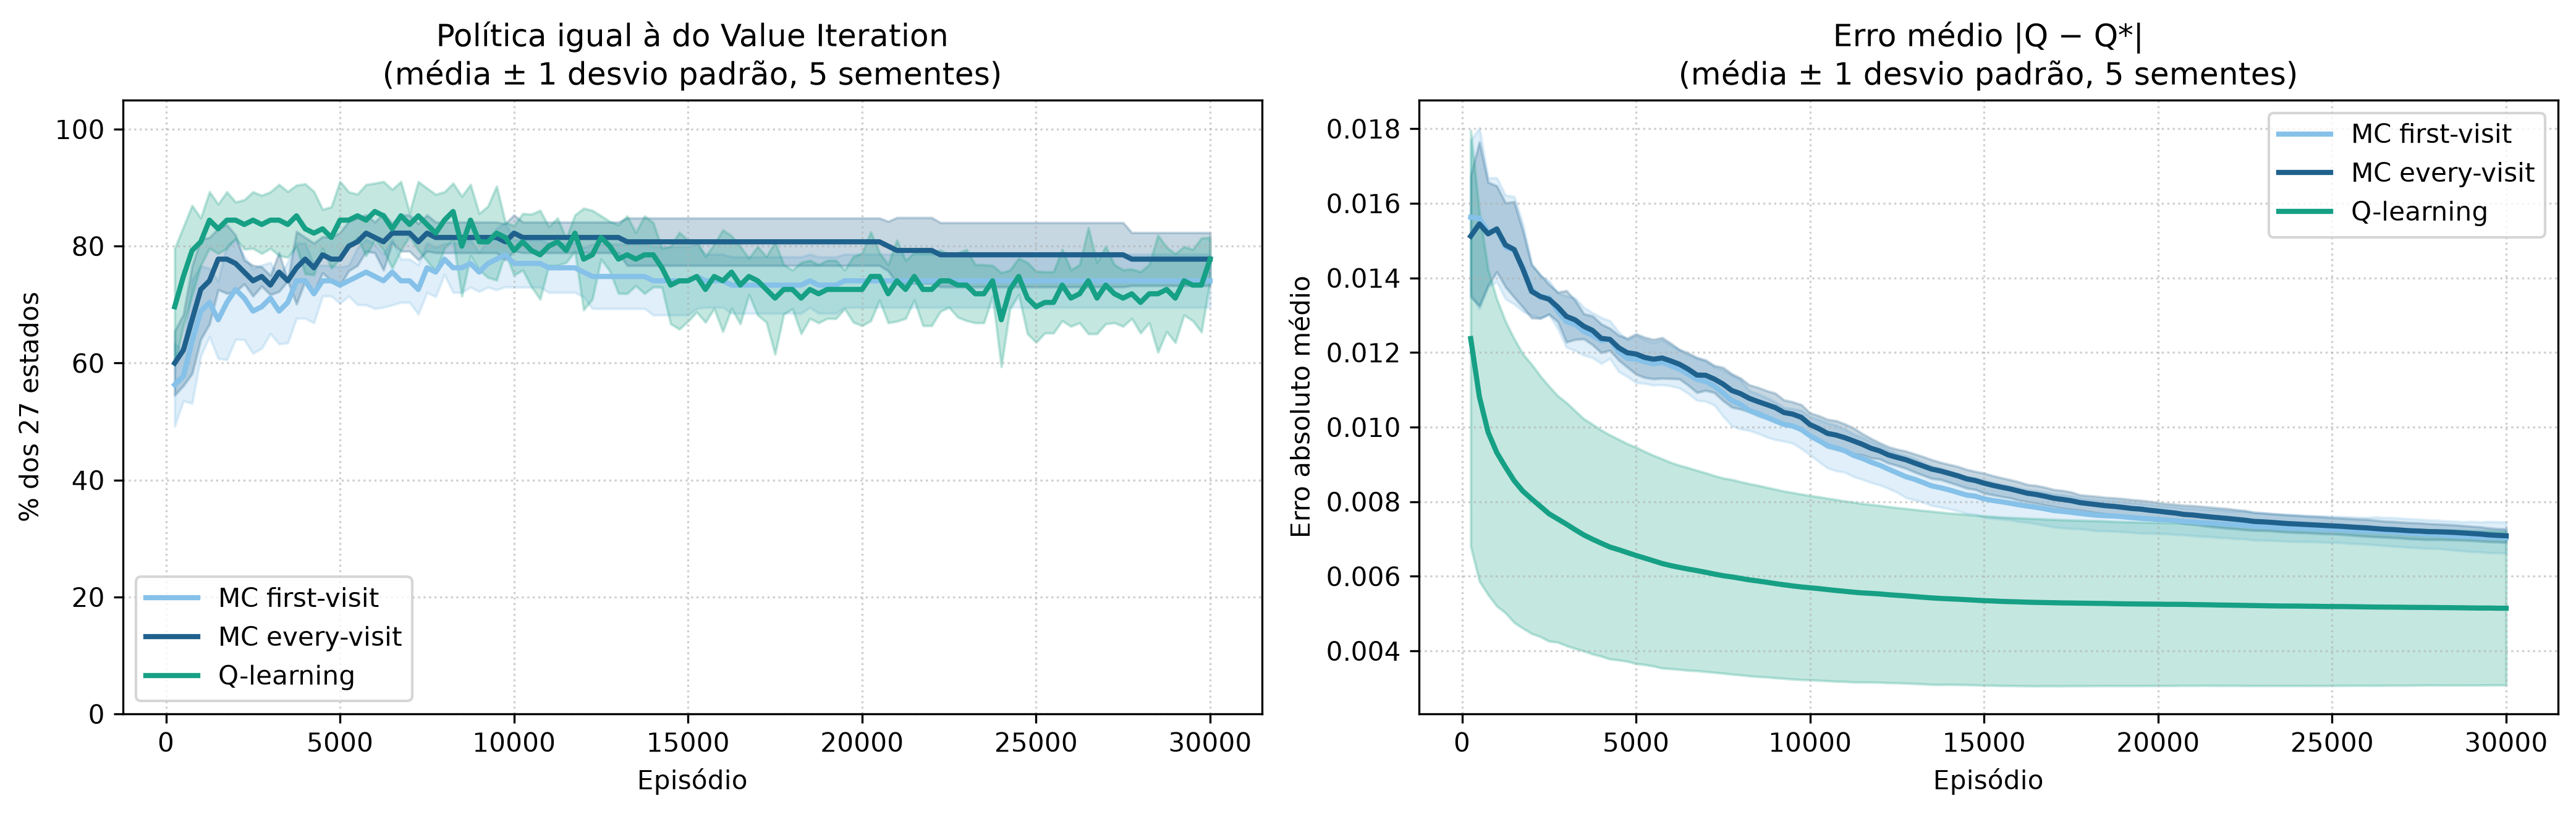
\includegraphics[width=\textwidth]{curva_sementes.png}
  \caption{Convergência do Monte Carlo e do Q-learning em 5 sementes (média $\pm$ 1 desvio padrão). Esquerda: fração dos 27 estados em que a política coincide com a do \textit{Value Iteration}. Direita: erro médio $|Q - Q^*|$, com $Q^*$ do \textit{Value Iteration} no mesmo MDP como referência teórica.}
  \label{fig:convergencia}
\end{figure*}

A Tabela~\ref{tab:metodos} resume as diferenças entre os métodos. A Fig.~\ref{fig:convergencia} compara a convergência em 5 sementes (42 a 46), com o $Q^*$ do \textit{Value Iteration} como referência teórica. O Q-learning chega mais perto de $Q^*$ (erro médio de 0,005, contra 0,007 do Monte Carlo, na média das 5 sementes), mas varia mais entre as sementes. Nos dois métodos, a política final coincide com a do \textit{Value Iteration} em cerca de três quartos dos estados.

Com a semente 42, os três métodos escolhem a mesma ação em 20 dos 27 estados, e Monte Carlo e Q-learning concordam entre si em 24. Todos coincidem nos regimes de alta; as diferenças se concentram perto da baixa e no regime neutro. No neutro estável sem posição aberta, por exemplo, o Q-learning compra, enquanto o \textit{Value Iteration} e o Monte Carlo ficam fora do mercado.

% =============================================================
\section{Protocolo Experimental}
\label{sec:metodologia}

\subsection{Simulador}

As políticas aprendidas são executadas no \texttt{gym-trading-env}~\cite{gymtrading}, com patrimônio inicial de US\$ 1.000, posições $\{-1, 0, +1\}$, corretagem $\kappa = 0{,}1\%$ e sem custo de aluguel na posição vendida. A cada dia, a política recebe as faixas $(\phi(x_t), \phi(x_{t-1}))$ e a posição anterior, e devolve a nova posição. Salvo indicação em contrário, as políticas são executadas de forma gulosa. O simulador não rebalanceia para $-100\%$, a cada dia, a posição vendida mantida; por isso, sua recompensa difere levemente de~\eqref{eq:recompensa} nesses passos.

\subsection{Métricas}

Seja $r^f_t = \ln(1 + i_t)/365$ a taxa livre de risco diária, em que $i_t$ é a taxa anual do T-bill americano de 3 meses (média de 0,78\% a.a. no treino e 3,94\% a.a. no teste). O índice de Sharpe~\cite{sharpe1966} anualizado usa o excesso de log-retorno $e_t = \ln(W_t / W_{t-1}) - r^f_t$:
\begin{equation}
  S = \sqrt{365}\; \frac{\bar{e}}{\sigma_e}.
\end{equation}
O \textit{drawdown} máximo (MDD) é a maior queda do patrimônio em relação ao pico anterior,
\begin{equation}
  \mathrm{MDD} = \min_t \left(\frac{W_t}{P_t} - 1\right), \qquad P_t = \max_{u \le t} W_u,
\end{equation}
e o índice de Calmar~\cite{young1991} é a razão entre o retorno anualizado $R_{\mathrm{anual}} = (W_T / W_0)^{365/T} - 1$ e $|\mathrm{MDD}|$. Também se reporta o número de trocas de posição. Como o caixa não rende juros no simulador, o Sharpe de estratégias que ficam muito tempo fora do mercado é conservador.

\subsection{Referências e Modelos Econométricos}

As políticas de RL são comparadas com três referências simples: \textit{Buy \& Hold} (sempre comprado), fora do mercado (sempre neutro) e uma política aleatória, que sorteia a ação a cada dia. Também são comparadas com modelos econométricos clássicos de previsão de retornos~\cite{campbell1997,tsay2010}:
\begin{itemize}
  \item passeio aleatório, que, com média positiva, equivale ao \textit{Buy \& Hold};
  \item AR(1) e ARMA(1,1) sobre $\rho_t$;
  \item regressão preditiva por mínimos quadrados (OLS), com $z_t = (x_t, \sigma_{20,t}, \rho_t, \rho_{t-1})$, em que $\sigma_{20,t}$ é a volatilidade de 20 dias;
  \item Logit e Probit para $P(\rho_{t+1} > 0)$, com as mesmas variáveis.
\end{itemize}
Todos são estimados apenas no treino, com a biblioteca \texttt{statsmodels}~\cite{statsmodels}, e a previsão vira posição: previsão de alta (retorno esperado positivo ou probabilidade de alta acima de 50\%) leva a comprado; caso contrário, a vendido. Para comparar todos nas mesmas condições, esse \textit{benchmark} usa um simulador próprio, com a fórmula~\eqref{eq:recompensa} e a mesma corretagem para todos; por isso, os números do RL diferem levemente dos do \texttt{gym-trading-env}.

\subsection{Validação \textit{Walk-forward}}

Na avaliação principal, cada modelo é estimado uma única vez, com dados até 31/12/2021, e usado no teste inteiro. Na validação \textit{walk-forward}~\cite{pardo2008}, os modelos são reestimados periodicamente, só com os dados disponíveis em cada data: tercis, $\hat{P}$, $\hat{R}$, \textit{Value Iteration}, Monte Carlo, Q-learning e modelos econométricos. Foram testadas sete configurações: sem reestimação, ou reestimação a cada 3, 6 ou 12 meses, com janela expansiva (todo o histórico) ou móvel (últimos 4 anos). Para não escolher pelo teste, cada modelo fica com a configuração de maior Sharpe numa validação dentro do treino, com estimação até 2018 e avaliação em 2019--2021. Monte Carlo e Q-learning usam a semente principal.

\subsection{Escolha do Fator de Desconto}
\label{sec:gamma}

O fator de desconto define o objetivo do agente, e não apenas a velocidade de convergência. Como a soma das recompensas é o log do patrimônio final, maximizar a carteira exige valorizar o futuro: $\gamma$ próximo de 1 aproxima o critério de Kelly~\cite{kelly1956}, enquanto $\gamma$ baixo torna o agente quase míope. Com $\gamma = 0{,}3$, a recompensa de daqui a cinco dias pesa $0{,}3^5 = 0{,}2\%$; com $\gamma = 0{,}8$, pesa $32{,}8\%$. Por isso, $\gamma = 0{,}8$ foi fixado antes, pelo objetivo, e a bateria de validação a seguir serve apenas para conferir a sensibilidade dessa escolha.

\begin{table}[!t]
  \centering
  \caption{Sharpe na validação (estimação até 2018, avaliação em 2019--2021) para cada $\gamma$; Monte Carlo e Q-learning na média de 5 sementes}
  \label{tab:gamma}
  \footnotesize
  \setlength{\tabcolsep}{4.5pt}
  \renewcommand{\arraystretch}{1.1}
  \begin{tabular}{c c c cccc}
    \toprule
    $\gamma$ & $\gamma^5$ & Episódio (dias) & VI & MC & QL & Média \\
    \midrule
    0,3  & 0,2\%  & 16  & 1,70 & 1,67 & 1,69 & 1,69 \\
    0,5  & 3,1\%  & 28  & 1,70 & 1,67 & 1,57 & 1,65 \\
    0,7  & 16,8\% & 52  & 1,59 & 1,54 & 1,40 & 1,51 \\
    \midrule
    \textbf{0,8} & \textbf{32,8\%} & \textbf{84} & \textbf{1,59} & \textbf{1,42} & \textbf{1,20} & \textbf{1,40} \\
    0,9  & 59,0\% & 176 & 1,59 & 1,17 & 1,16 & 1,31 \\
    0,95 & 77,4\% & 360 & 1,59 & 1,18 & 1,17 & 1,31 \\
    \bottomrule
  \end{tabular}
\end{table}

Para conferir a escolha sem usar o teste, todo o procedimento foi repetido com $\gamma$ igual a 0,3, 0,5, 0,7, 0,8, 0,9 e 0,95, com estimação até 2018, avaliação em 2019--2021, horizonte $H$ ajustado a cada $\gamma$ e Monte Carlo e Q-learning repetidos com 5 sementes (Tabela~\ref{tab:gamma}). Valores menores de $\gamma$ têm Sharpe maior na validação, mas olham apenas um ou dois dias à frente. Entre os $\gamma \ge 0{,}8$, o maior Sharpe médio é o de $\gamma = 0{,}8$ (1,40), e o \textit{Value Iteration} quase não muda com $\gamma$. Os valores da validação não são comparáveis aos do teste: o período é outro e a estimação vai só até 2018. No teste, consultado só por transparência, o Sharpe do \textit{Value Iteration} é o mesmo (0,46) para todo $\gamma \le 0{,}8$, e o Q-learning é o método mais sensível a $\gamma$.

% =============================================================
\section{Resultados}
\label{sec:resultados}

\begin{table*}[!t]
  \centering
  \caption{Resultados no \texttt{gym-trading-env} com $\kappa = 0{,}1\%$ e $\gamma = 0{,}8$ (Monte Carlo \textit{every-visit} e Q-learning com a semente 42)}
  \label{tab:resultados}
  \footnotesize
  \setlength{\tabcolsep}{8pt}
  \renewcommand{\arraystretch}{1.1}
  \begin{tabular}{l cccccc}
    \toprule
    \textbf{Estratégia} & \textbf{Retorno total} & \textbf{Retorno anual} & \textbf{Sharpe} & \textbf{MDD} & \textbf{Calmar} & \textbf{Trocas} \\
    \midrule
    \multicolumn{7}{l}{\textit{Teste (2022 a 2026)}} \\
    MDP (\textit{Value Iteration}) & 127,80\%     & 18,37\%      & 0,46      & $-$29,35\% & 0,63      & 113 \\
    Monte Carlo                    & 119,47\%     & 17,47\%      & 0,44      & $-$26,95\% & 0,65      & 108 \\
    Q-learning                     & 86,39\%      & 13,60\%      & 0,26      & $-$51,25\% & 0,27      & 190 \\
    \textit{Buy \& Hold}           & 31,95\%      & 5,84\%       & 0,04      & $-$66,93\% & 0,09      & 1 \\
    Fora do mercado                & 0,00\%       & 0,00\%       & 0,00      & 0,00\%     & --        & 0 \\
    Aleatória                      & $-$93,85\%   & $-$43,52\%   & $-$1,45   & $-$94,58\% & $-$0,46   & 1.163 \\
    \midrule
    \multicolumn{7}{l}{\textit{Treino (2014 a 2021)}} \\
    MDP (\textit{Value Iteration}) & 6.947,44\%   & 81,24\%      & 1,09      & $-$50,59\% & 1,61      & 140 \\
    Monte Carlo                    & 9.802,30\%   & 90,06\%      & 1,20      & $-$52,95\% & 1,70      & 119 \\
    Q-learning                     & 26.866,84\%  & 118,62\%     & 1,37      & $-$69,05\% & 1,72      & 195 \\
    \textit{Buy \& Hold}           & 13.144,05\%  & 97,94\%      & 0,90      & $-$83,40\% & 1,17      & 1 \\
    Fora do mercado                & 0,00\%       & 0,00\%       & 0,00      & 0,00\%     & --        & 0 \\
    Aleatória                      & $-$88,73\%   & $-$26,29\%   & $-$0,52   & $-$95,74\% & $-$0,27   & 1.721 \\
    \bottomrule
  \end{tabular}
\end{table*}

\begin{table*}[!t]
  \centering
  \caption{\textit{Benchmark} no teste (2022 a 2026): RL $\times$ modelos econométricos, ordenados pelo Sharpe, no simulador próprio}
  \label{tab:benchmark}
  \footnotesize
  \setlength{\tabcolsep}{10pt}
  \renewcommand{\arraystretch}{1.1}
  \begin{tabular}{l ccccc}
    \toprule
    \textbf{Modelo} & \textbf{Retorno total} & \textbf{Sharpe} & \textbf{MDD} & \textbf{Calmar} & \textbf{Trocas} \\
    \midrule
    \textbf{MDP (\textit{Value Iteration})}   & \textbf{+126,86\%} & \textbf{0,46} & \textbf{$-$29,35\%} & \textbf{0,62} & \textbf{113} \\
    \textbf{Monte Carlo}                      & \textbf{+119,46\%} & \textbf{0,44} & \textbf{$-$26,95\%} & \textbf{0,65} & \textbf{108} \\
    \textbf{Q-learning}                       & \textbf{+86,08\%}  & \textbf{0,26} & \textbf{$-$51,28\%} & \textbf{0,26} & \textbf{190} \\
    \midrule
    AR(1)                                     & +110,82\%          & 0,23          & $-$73,07\%          & 0,23          & 49  \\
    ARMA(1,1)                                 & +100,18\%          & 0,21          & $-$72,85\%          & 0,21          & 43  \\
    Probit                                    & +54,51\%           & 0,10          & $-$72,95\%          & 0,13          & 113 \\
    Logit                                     & +50,53\%           & 0,09          & $-$72,95\%          & 0,12          & 115 \\
    Passeio aleatório (\textit{Buy \& Hold})  & +31,95\%           & 0,04          & $-$66,93\%          & 0,09          & 1   \\
    Regressão preditiva (OLS)                 & $-$48,48\%         & $-$0,35       & $-$77,59\%          & $-$0,16       & 225 \\
    \bottomrule
  \end{tabular}
\end{table*}

\subsection{Desempenho no Teste}

A Tabela~\ref{tab:resultados} reúne os resultados no simulador. No teste, o \textit{Value Iteration} obteve o maior Sharpe (0,46) e retorno total de 127,80\%, com MDD de $-29{,}35\%$. Sem conhecer o modelo, o Monte Carlo ficou muito próximo, com Sharpe de 0,44 e o menor MDD ($-26{,}95\%$). O Q-learning teve Sharpe de 0,26, mais trocas (190) e MDD de $-51{,}25\%$.

O teste começa perto de um topo: o BTC caiu de cerca de US\$ 47 mil em janeiro de 2022 para cerca de US\$ 16 mil no fim de 2022 (Fig.~\ref{fig:teste}). Por isso, o \textit{Buy \& Hold} rendeu só 31,95\%, com Sharpe de 0,04 e MDD de $-66{,}93\%$. As três políticas de RL superaram o \textit{Buy \& Hold} em retorno, Sharpe e MDD, e a política aleatória perdeu 93,85\%. No treino, o Q-learning teve o maior Sharpe (1,37), acima do Monte Carlo (1,20) e do \textit{Value Iteration} (1,09), mas foi o pior dos três no teste (Seção~\ref{sec:discussao}).

\begin{figure}[!t]
  \centering
  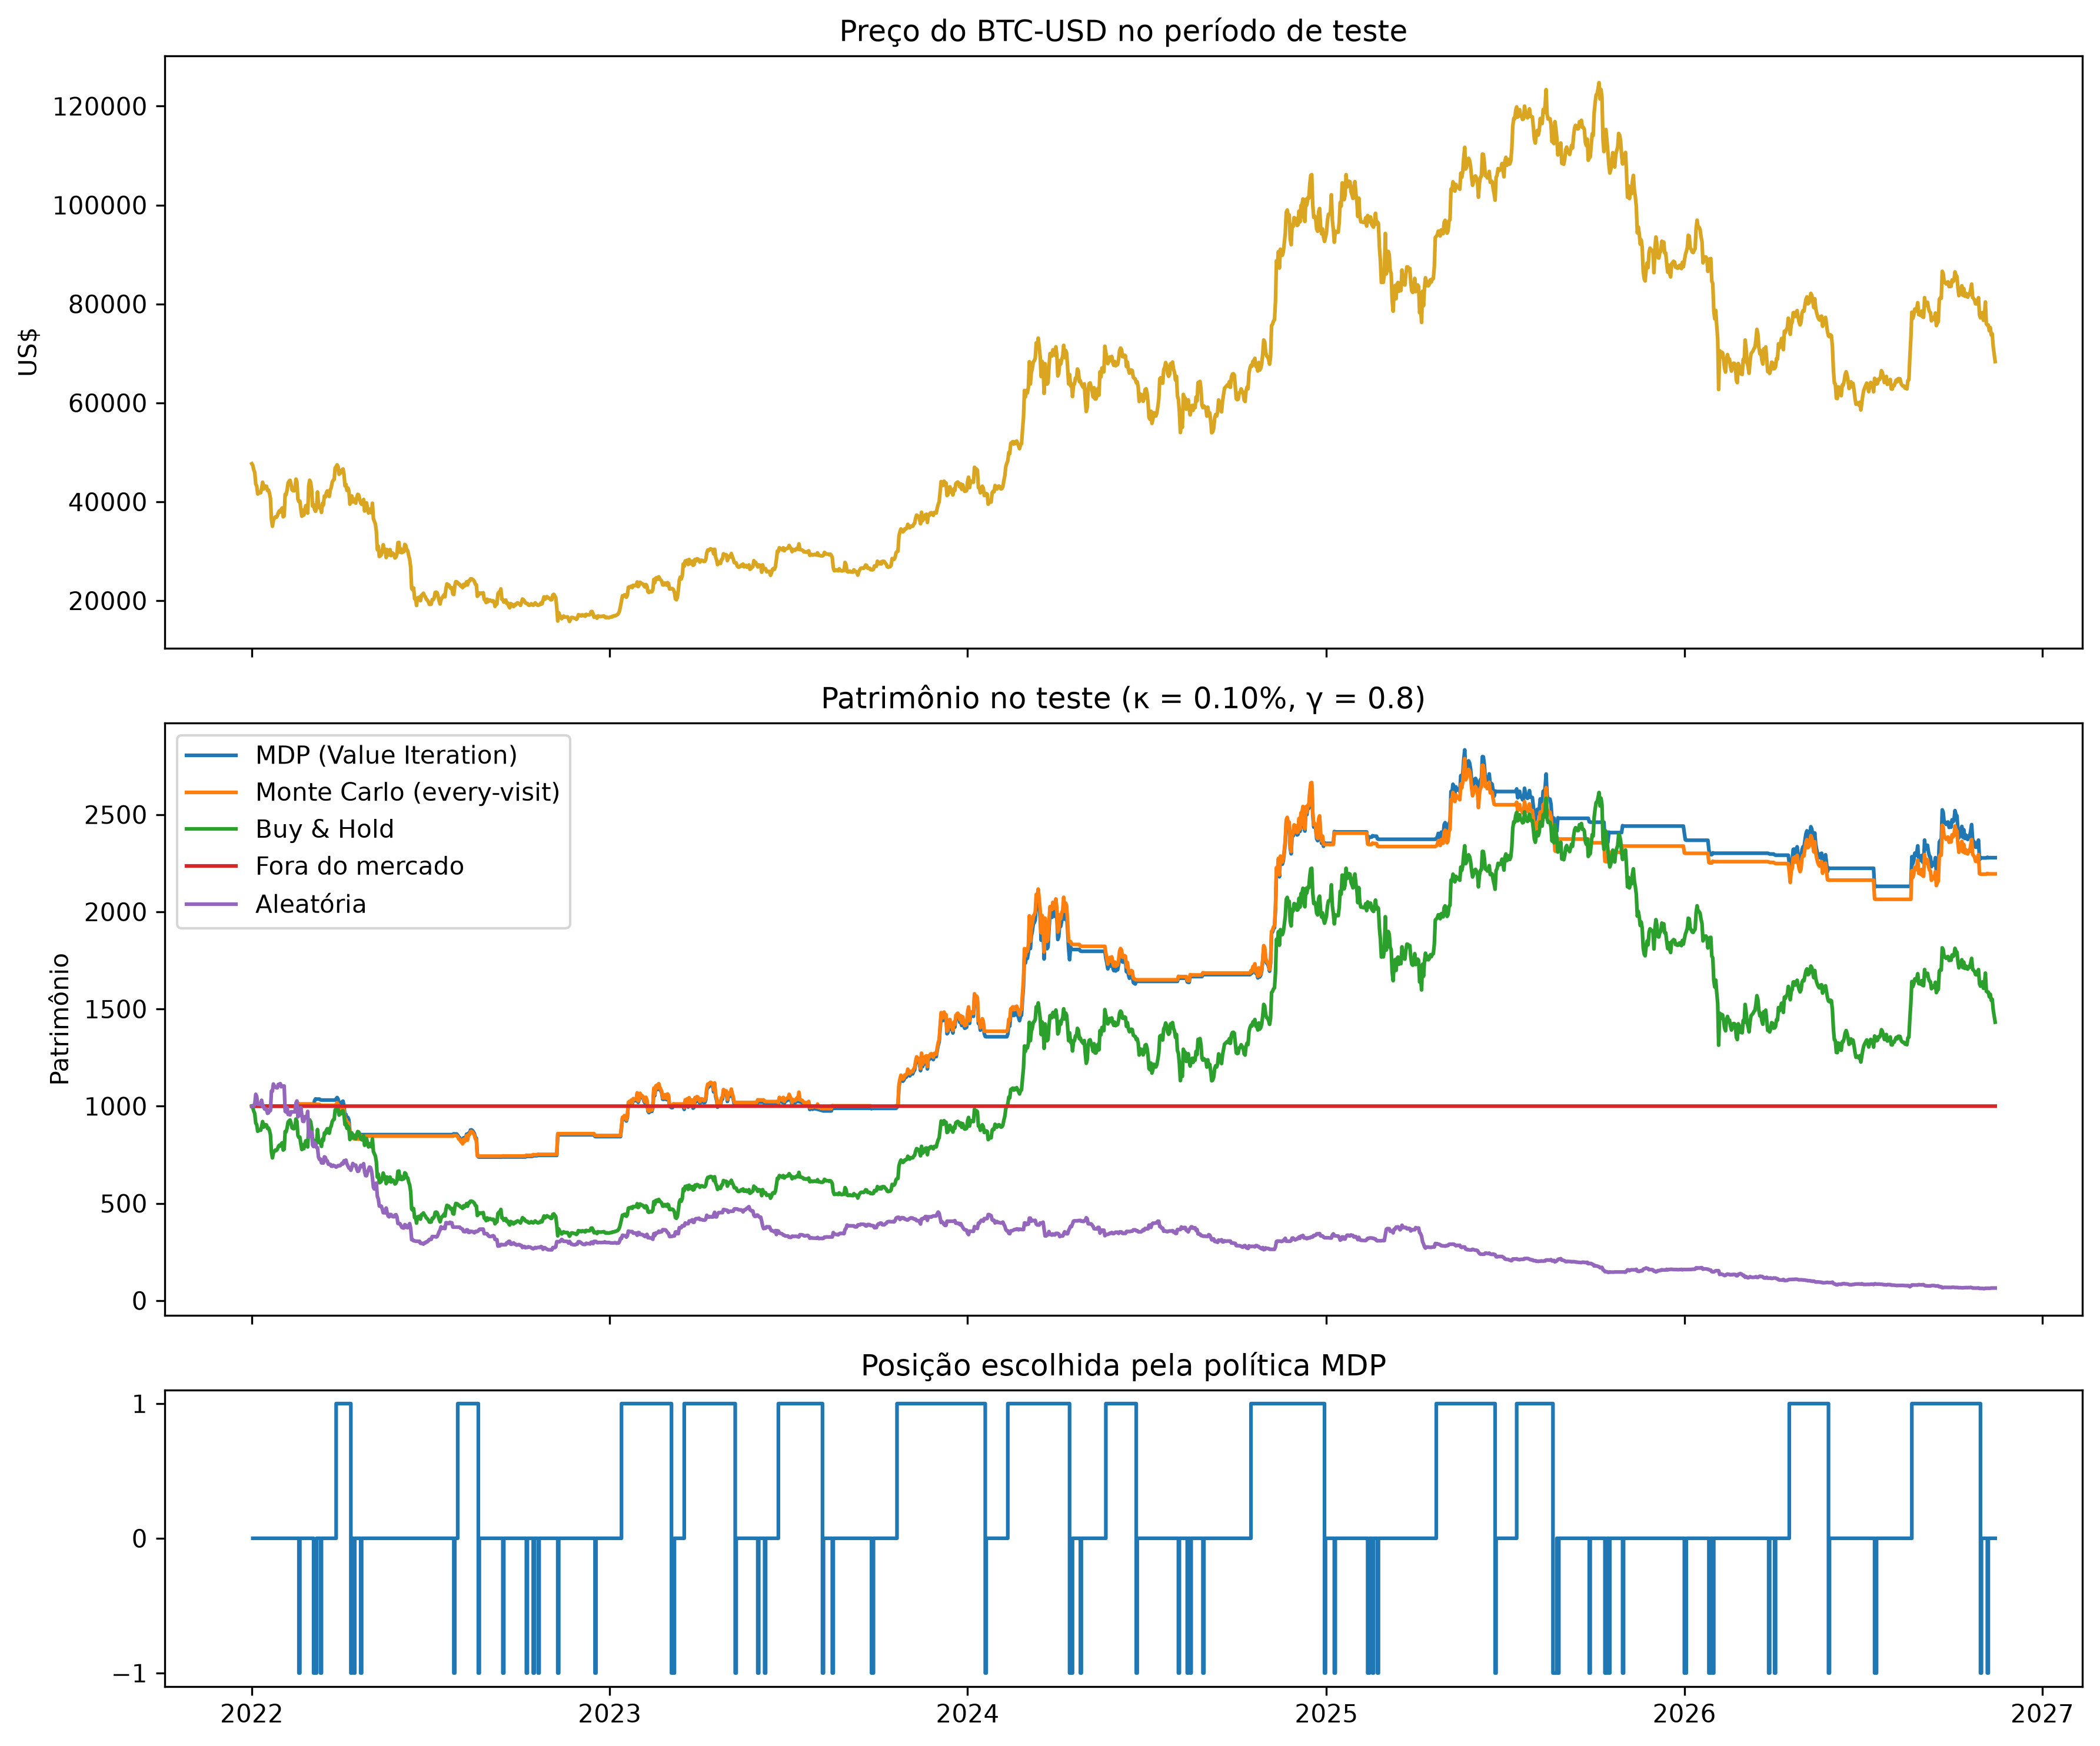
\includegraphics[width=\columnwidth]{grafico_teste.png}
  \caption{Teste (2022--2026): preço do BTC-USD (topo), patrimônio das estratégias com $\kappa = 0{,}1\%$ e $\gamma = 0{,}8$ (meio) e posição escolhida pela política do \textit{Value Iteration} (base).}
  \label{fig:teste}
\end{figure}

\subsection{Efeito da Corretagem}

Para isolar o custo das trocas, as mesmas políticas foram executadas sem corretagem (Tabela~\ref{tab:corretagem}). Como as ações são idênticas, a diferença é só o custo. Quem troca mais paga mais: o Q-learning perde 4,51 pontos percentuais de retorno anual com a corretagem, contra 3,09 do \textit{Value Iteration} e 2,62 do Monte Carlo. A ordem entre as estratégias não muda.

\begin{table}[!t]
  \centering
  \caption{Teste com e sem corretagem: mesmas políticas e mesmas ações}
  \label{tab:corretagem}
  \footnotesize
  \setlength{\tabcolsep}{4.5pt}
  \renewcommand{\arraystretch}{1.1}
  \begin{tabular}{l cccc}
    \toprule
    & & \multicolumn{2}{c}{\textbf{Sharpe}} & \textbf{Custo} \\
    \cmidrule(lr){3-4}
    \textbf{Estratégia} & \textbf{Trocas} & \textbf{com} & \textbf{sem} & \textbf{(p.p. ao ano)} \\
    \midrule
    MDP (VI)              & 113   & 0,46    & 0,55    & 3,09  \\
    Monte Carlo           & 108   & 0,44    & 0,51    & 2,62  \\
    Q-learning            & 190   & 0,26    & 0,37    & 4,51  \\
    \textit{Buy \& Hold}  & 1     & 0,04    & 0,04    & 0,02  \\
    Aleatória             & 1.163 & $-$1,45 & $-$0,68 & 21,54 \\
    \bottomrule
  \end{tabular}
\end{table}

\subsection{Política Gulosa $\times$ $\varepsilon$-gulosa}

Executar as políticas com exploração ($\varepsilon = 0{,}1$, média de 100 sementes) piorou os três métodos (Tabela~\ref{tab:epsilon}). O Sharpe do \textit{Value Iteration} cai de 0,46 para 0,20, e o número de trocas mais que dobra. A versão $\varepsilon$-gulosa superou a gulosa em apenas 21\% a 24\% das sementes: a exploração serve para aprender, não para operar.

\begin{table}[!t]
  \centering
  \caption{Teste com política gulosa e $\varepsilon$-gulosa ($\varepsilon = 0{,}1$, média de 100 sementes)}
  \label{tab:epsilon}
  \footnotesize
  \setlength{\tabcolsep}{4.5pt}
  \renewcommand{\arraystretch}{1.1}
  \begin{tabular}{l cccc}
    \toprule
    \textbf{Política} & \textbf{Sharpe} & \textbf{MDD} & \textbf{Trocas} & \textbf{$\varepsilon$ vence} \\
    \midrule
    MDP: gulosa                         & 0,46 & $-$29,35\% & 113 & --    \\
    MDP: $\varepsilon$-gulosa           & 0,20 & $-$49,87\% & 286 & 24\%  \\
    \midrule
    Monte Carlo: gulosa                 & 0,44 & $-$26,95\% & 108 & --    \\
    Monte Carlo: $\varepsilon$-gulosa   & 0,14 & $-$50,67\% & 289 & 21\%  \\
    \midrule
    Q-learning: gulosa                  & 0,26 & $-$51,25\% & 190 & --    \\
    Q-learning: $\varepsilon$-gulosa    & 0,04 & $-$59,22\% & 373 & 23\%  \\
    \bottomrule
  \end{tabular}
\end{table}

\subsection{Variabilidade entre Sementes}

Os resultados acima usam a semente 42. A Tabela~\ref{tab:sementes} repete Monte Carlo e Q-learning com 5 sementes (42 a 46). O Monte Carlo \textit{every-visit} é o mais estável, com desvio padrão de 0,09 no Sharpe do teste. Na média, o \textit{first-visit} tem Sharpe de treino maior (1,42 contra 1,17): com uma única semente, a escolha da versão do Monte Carlo dependeu da sorte, embora o \textit{every-visit} tenha Sharpe médio maior e muito menos variância no teste. O Q-learning escolhe a mesma ação nas 5 sementes em 21 dos 27 estados e tem Sharpe médio de 0,24 no teste.

\begin{table}[!t]
  \centering
  \caption{Monte Carlo e Q-learning com 5 sementes (42 a 46): média (desvio padrão)}
  \label{tab:sementes}
  \footnotesize
  \setlength{\tabcolsep}{4pt}
  \renewcommand{\arraystretch}{1.1}
  \begin{tabular}{l ccc}
    \toprule
    & \textbf{Treino} & \multicolumn{2}{c}{\textbf{Teste}} \\
    \cmidrule(lr){2-2} \cmidrule(lr){3-4}
    \textbf{Método} & \textbf{Sharpe} & \textbf{Sharpe} & \textbf{MDD} \\
    \midrule
    MC \textit{first-visit}  & 1,42 (0,17) & 0,30 (0,26) & $-$39,07\% (19,31) \\
    MC \textit{every-visit}  & 1,17 (0,04) & 0,34 (0,09) & $-$33,24\% (7,94)  \\
    Q-learning               & 1,31 (0,10) & 0,24 (0,12) & $-$49,58\% (13,24) \\
    \bottomrule
  \end{tabular}
\end{table}

\subsection{Comparação com Modelos Econométricos}

Na comparação com os modelos econométricos (Tabela~\ref{tab:benchmark}), as três políticas de RL lideram em Sharpe e Calmar. O melhor modelo econométrico, o AR(1), tem Sharpe de 0,23 e MDD de $-73{,}07\%$; \textit{Value Iteration} e Monte Carlo têm menos da metade dessa queda máxima. A regressão preditiva perde 48,48\%. As pequenas diferenças entre os números do RL nas Tabelas~\ref{tab:resultados} e~\ref{tab:benchmark} vêm dos simuladores: o \texttt{gym-trading-env} não rebalanceia a posição vendida mantida.

\subsection{\textit{Walk-forward}}

Com janela expansiva, retreinar não melhorou nenhum modelo no teste (Tabela~\ref{tab:walkforward}). A validação escolheu não reestimar o \textit{Value Iteration}, que manteve o Sharpe de 0,46. Para Monte Carlo e Q-learning, escolheu reestimar a cada 3 meses, o que levou a Sharpe de 0,26 e $-0{,}17$ no teste. A única melhora em relação ao treino único ocorreu no Q-learning com janela móvel de 4 anos e reestimação anual (Sharpe 0,33, com uma semente), configuração que a validação não escolheu.

\begin{table}[!t]
  \centering
  \caption{\textit{Walk-forward}: Sharpe no teste reestimando com todo o histórico e configuração escolhida na validação (2019--2021)}
  \label{tab:walkforward}
  \footnotesize
  \setlength{\tabcolsep}{4pt}
  \renewcommand{\arraystretch}{1.1}
  \begin{tabular}{l c ccc c}
    \toprule
    & & \multicolumn{3}{c}{\textbf{Reestima a cada}} & \\
    \cmidrule(lr){3-5}
    \textbf{Modelo} & \textbf{Nunca} & \textbf{12 m} & \textbf{6 m} & \textbf{3 m} & \textbf{Escolha} \\
    \midrule
    MDP (VI)              & 0,46 & 0,28    & 0,35 & 0,07    & nunca    \\
    Monte Carlo           & 0,44 & 0,14    & 0,18 & 0,26    & 3 meses  \\
    Q-learning            & 0,26 & $-$0,03 & 0,25 & $-$0,17 & 3 meses  \\
    AR(1)                 & 0,23 & 0,18    & 0,06 & 0,06    & 12 meses \\
    \textit{Buy \& Hold}  & 0,04 & 0,04    & 0,04 & 0,04    & --       \\
    \bottomrule
  \end{tabular}
\end{table}

% =============================================================
\section{Discussão}
\label{sec:discussao}

\textit{Por que o Q-learning foi pior?} Três fatores se somam. Primeiro, ele aprendeu a comprar no regime neutro estável mesmo sem posição aberta. Esse comportamento foi premiado no treino, um período de forte alta do Bitcoin, mas prejudicou no teste, que começou com um mercado de baixa; isso explica o maior Sharpe no treino e o pior no teste. Segundo, ele troca mais de posição (190 trocas, contra 113 do \textit{Value Iteration}) e paga mais corretagem. Terceiro, o Q-learning depende da hipótese de Markov ao fazer \textit{bootstrap} pelo estado seguinte e está sujeito ao viés de maximização do operador $\max$~\cite{sutton2018}, enquanto o Monte Carlo usa o retorno real e é mais robusto a uma discretização apenas aproximadamente Markov. Estar mais perto de $Q^*$ também não garante a melhor política no teste: $Q^*$ é ótimo só para o modelo estimado no treino, e pequenas diferenças de valor entre ações bastam para mudar a ação escolhida.

\textit{Por que retreinar não ajudou?} Cada reestimação recalcula os tercis e as probabilidades de transição. Como as faixas são relativas ao histórico, o mesmo preço pode mudar de faixa depois de um retreino, e a política troca de ação em parte dos estados. Nesse experimento, a estabilidade da política original superou a adaptação a dados mais recentes, uma tensão típica entre acompanhar mudanças na distribuição dos dados e manter o modelo estável.

\textit{Limitações.} O estado é simples: três faixas do sinal preço/MA50 nos dois últimos dias, sem volatilidade, volume ou variáveis macroeconômicas, e por isso a propriedade de Markov é só aproximada. Há um único ativo e um único corte entre treino e teste. Os custos são simplificados: só corretagem fixa, sem \textit{slippage}, impacto de mercado ou aluguel na posição vendida. O caixa não rende juros no simulador, e a posição vendida mantida não é rebalanceada. Resultados passados não garantem desempenho futuro.

% =============================================================
\section{Conclusão}
\label{sec:conclusao}

Este trabalho transformou uma série financeira contínua e ruidosa em um MDP finito de 27 estados e o resolveu por três caminhos. Com o modelo estimado, a cadeia
\begin{equation}
  (\hat{P}, \hat{R}) \longrightarrow V^* \longrightarrow \pi^*
\end{equation}
converge em 98 iterações e produz uma política interpretável, que cabe numa tabela, com o melhor desempenho no teste: Sharpe de 0,46, contra 0,04 do \textit{Buy \& Hold}. Sem modelo, o Monte Carlo chegou perto desse resultado (0,44), e o Q-learning, embora mais próximo de $Q^*$, foi o mais sensível ao período de treino. As três políticas superaram os modelos econométricos em Sharpe e Calmar.

Ao definir a recompensa como o log-retorno da carteira, a política obtida é ótima, no modelo estimado, para o crescimento composto do capital, e $\gamma = 0{,}8$ preserva esse objetivo sem tornar o agente míope. O desempenho real depende da validade aproximada da hipótese de Markov, do erro de estimação de $(\hat{P}, \hat{R})$ e da estabilidade do regime de mercado entre treino e teste, como mostraram o \textit{walk-forward} e a comparação entre sementes. Trabalhos futuros podem enriquecer o estado com volatilidade e volume, incluir outros ativos e usar custos mais realistas.

% =============================================================
\begin{thebibliography}{00}

\bibitem{sutton2018}
R.~S. Sutton and A.~G. Barto, \textit{Reinforcement Learning: An Introduction}, 2nd~ed. Cambridge, MA, USA: MIT Press, 2018.

\bibitem{moody1998}
J.~Moody, L.~Wu, Y.~Liao, and M.~Saffell, ``Performance functions and reinforcement learning for trading systems and portfolios,'' \textit{J. Forecasting}, vol.~17, no.~5--6, pp.~441--470, 1998.

\bibitem{moody2001}
J.~Moody and M.~Saffell, ``Learning to trade via direct reinforcement,'' \textit{IEEE Trans. Neural Netw.}, vol.~12, no.~4, pp.~875--889, 2001.

\bibitem{gymtrading}
C.~Perroud, ``Gym Trading Env,'' repositório GitHub. [Online]. Disponível em: \url{https://github.com/ClementPerroud/Gym-Trading-Env}

\bibitem{puterman1994}
M.~L. Puterman, \textit{Markov Decision Processes: Discrete Stochastic Dynamic Programming}. New York, NY, USA: Wiley, 1994.

\bibitem{kelly1956}
J.~L. Kelly, Jr., ``A new interpretation of information rate,'' \textit{Bell Syst. Tech. J.}, vol.~35, no.~4, pp.~917--926, 1956.

\bibitem{yfinance}
R.~Aroussi, ``yfinance,'' repositório GitHub. [Online]. Disponível em: \url{https://github.com/ranaroussi/yfinance}

\bibitem{campbell1997}
J.~Y. Campbell, A.~W. Lo, and A.~C. MacKinlay, \textit{The Econometrics of Financial Markets}. Princeton, NJ, USA: Princeton Univ. Press, 1997.

\bibitem{tsay2010}
R.~S. Tsay, \textit{Analysis of Financial Time Series}, 3rd~ed. Hoboken, NJ, USA: Wiley, 2010.

\bibitem{anderson1957}
T.~W. Anderson and L.~A. Goodman, ``Statistical inference about Markov chains,'' \textit{Ann. Math. Statist.}, vol.~28, no.~1, pp.~89--110, 1957.

\bibitem{bellman1957}
R.~Bellman, \textit{Dynamic Programming}. Princeton, NJ, USA: Princeton Univ. Press, 1957.

\bibitem{watkins1992}
C.~J. C.~H. Watkins and P.~Dayan, ``Q-learning,'' \textit{Mach. Learn.}, vol.~8, no.~3--4, pp.~279--292, 1992.

\bibitem{sharpe1966}
W.~F. Sharpe, ``Mutual fund performance,'' \textit{J. Bus.}, vol.~39, no.~1, pp.~119--138, 1966.

\bibitem{young1991}
T.~W. Young, ``Calmar ratio: A smoother tool,'' \textit{Futures}, vol.~20, no.~1, p.~40, 1991.

\bibitem{statsmodels}
S.~Seabold and J.~Perktold, ``Statsmodels: Econometric and statistical modeling with Python,'' in \textit{Proc. 9th Python Sci. Conf. (SciPy)}, 2010, pp.~92--96.

\bibitem{pardo2008}
R.~Pardo, \textit{The Evaluation and Optimization of Trading Strategies}, 2nd~ed. Hoboken, NJ, USA: Wiley, 2008.

\end{thebibliography}

\end{document}
